% Incomplete

\begin{enumerate}
    \item Consider the sample space given with outcomes $a$, $b$, $c$, $d$ and $e$. Calculate
    \begin{itemize}
        \item $P(b) = 1-P(a)-P(c)-P(d)-P(e) = 1 - 0.13-0.48-0.02-0.22 = 0.15$
        \item $P(A)=P(c)+P(d)=0.48+0.02 = 0.5$
        \item $P(A') = 1 - P(A) = 1-0.5 = 0.5$
    \end{itemize}

    \item Two fair dice are thrown, one red and one blue. What is the probability that the red die has a score that is strictly greater than the score of the blue die? Why is this probability less than 0.5? What is the complement of this event?\\
    The number of ways that the red die has a score that is strictly greater than the score of the blue die is the number of ways we can choose 2 distinct numbers from $\{1,2,3,4,5,6\}$, assign the bigger number to the red die and smaller one to the blue die. Hence:
    $$P(\n{red} > \n{blue}) = {6\choose2}/6^2 = 5/12$$
    This probability less than 0.5 because it excludes the result of the blue die's score being greater than \textbf{or equal} than the red die's score.
    The complement of this event is blue die's score being greater than \textbf{or equal} than the red die's score.
    
    \item If a card is chosen at random from a pack of cards, what is the probability that the card is from one of the 2 black suits?
    $$P(\n{black}) = 26/52 = 1/2$$

    \item A fair coin is tossed 3 times. What is the probability that 2 heads will be obtained in \textit{succession}?
    $$P(\n{2 head succession}) = \frac{|\{(h,h,h),(h,h,t),(t,h,h)\}|}{2^3} = 3/8$$

    \item Consider the sample space $\mathcal{S}$ = \{0, 1, 2\} and the event $A=\{0\}$. Explain why $A\ne\emptyset$.\\
    Because $A=\{0\}\ne\emptyset$.

    \item Consider the sample space and events given by the figure
    \begin{enumerate}
        \item $P(B)=0.08+0.13+0.06+0.01+0.02+0.05+0.11=0.46$
        \item $P(B\cap C)=0.02 + 0.05 + 0.11=0.18$
        \item $P(A\cap C)=0.07 + 0.05+0.01+0.02+0.05+0.08+0.04+0.07+0.11=0.5$
        \item $P(A\cap B \cap C) = 0.02 + 0.07 = 0.07$
        \item $P(A\cup B\cup C)=1-0.04-0.05-0.03=0.88$
        \item $P(A'\cap B)=P(B) - P(A\cap B)=0.46-0.01-0.02-0.05=0.38$
        \item $P(B'\cup C)=1-P(B)+P(B\cap C) = 1-0.46+0.18=0.72$
        \item $P(A\cup(B\cap C))= 0.07+0.05+0.01+0.02+0.05+0.08+0.04+0.11=0.43$
        \item $P((A\cup B)\cap C)=0.11+0.02+0.05+0.08+0.04=0.3$
        \item $P((A'\cup C)')=0.05+0.01+0.07=0.13$
    \end{enumerate}

    \item Use Venn diagrams to illustrate the equations:
    \begin{center}
        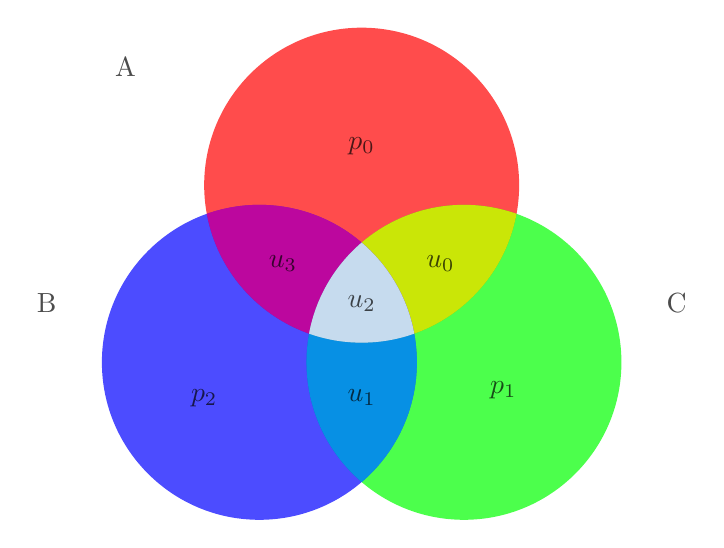
\begin{tikzpicture}[thin,fill opacity=0.7]
        \draw [draw=none, fill=red] (90:1.5) circle (2cm);
        \draw [draw=none, fill=green] (-30:1.5) circle (2cm);
        \draw [draw=none, fill=blue] (210:1.5) circle (2cm);
        \begin{scope}
            \clip (90:1.5) circle(2cm);
            \draw [draw=none, fill=yellow] (-30:1.5) circle (2cm);
        \end{scope}
        \begin{scope}
            \clip (210:1.5) circle(2cm);
            \draw [draw=none, fill=magenta] (90:1.5) circle (2cm);
        \end{scope}
        \node at (-3,3) {A};
        \node at (-4,0) {B};
        \node at (4,0) {C};
        \begin{scope}
            \clip (-30:1.5) circle(2cm);
            \draw [draw=none, fill=cyan] (210:1.5) circle (2cm);
        \end{scope}
        \begin{scope}
            \clip (90:1.5) circle(2cm);
            \clip (210:1.5) circle(2cm);
            \draw [draw=none, fill=white] (-30:1.5) circle (2cm);	
        \end{scope}
        \node at (1,.5) {$u_0$};
        \node at (0,0) {$u_2$};
        \node at (1.8,-1.1) {$p_1$};
        \node at (-1,.5) {$u_3$};
        \node at (0,-1.2) {$u_1$};
        \node at (0,2) {$p_0$};
        \node at (-2,-1.2) {$p_2$};
        \end{tikzpicture}
    \end{center}
    \begin{enumerate}
        \item $A\cup  (B\cap C)=(A\cup B)\cap (A\cup C)$
        \item $A\cap (B\cup  C)=(A\cap B)\cup  (A\cap C)$
        \item $(A\cap B\cap C)' =A'\cup  B'\cup  C'$
    \end{enumerate}
    
    \item In a study of patients arriving at a hospital emergency room, the gender of the patients is considered, together with whether the patients are younger or older than 30 years of age, and whether or not the patients are admitted to the hospital. It is found that 45\% of the patients are male, 30\% of the patients are younger than 30 years of age, 15\% of the patients are females older than 30 years of age who are admitted to the hospital and 21\% of the patients are females younger than 30 years of age. What proportion of the patients are females older than 30 years of age who are not admitted to the hospital?
    
\end{enumerate}